% !TEX root = ../main.tex

As mentioned earlier, poorly implemented smart contracts can be exploited in several ways which, in some cases, can result in enormous security attacks. \textit{The re-entrancy attack} is among those high severity security issues that resulted the attack on The DAO system, Decentralized Autonomous Organization in 2016\footnote{\url{https://github.com/slockit/DAO.}}. The DAO was a form of investor-directed venture capital fund with an objective to facilitate fundraising on new ideas or new projects through crowdfunding; providing the owners with tokens, which then enable them to vote for their favourite ideas and projects. However, due to the poor design of The Dao smart contract, attackers managed to drain 86 million USD~\cite{A50Milli86:online} off its funds. Following sections explain the overview of the DAO attack.

\subsubsection{Attack Analysis}
Code~\ref{code:dao} is a simplified version of the DAO smart contract, which is vulnerable to the reentrancy attack. In order to interact with the DAO, a user first donates some Ethers to the DAO smart contract using the donate() function and the contract updates the user’s balance with the exact amount it has received (Code~\ref{code:dao} , line 6). At this point, user can withdraw the funds back by calling the withdraw() function (Code~\ref{code:dao} , line 12). Doing so, the DAO contract sends funds back to the user (msg.sender) using the msg.sender.call.value(amount)() (Code~\ref{code:dao} , line 16). The issue is that, the DAO smart contract first transfers the funds to the user (msg.sender) and then updates his account balance. This makes the reentrancy attack possible as a malicious user can drain funds from the contract by recursively calling the withdraw() function before the contract’s state (user’s balance) gets updated. To do so, attacker has to define a payable fallback() function in his smart contract. Followings explain the details of the fallback() function and how it was used in the actual DAO attack.

\textbf{Fallback() Function:} In Solidity programming language, a fallback() function is referred to an unnamed function, without any arguments and return value. This function gets executed automatically every time the smart contract receives Ether without any data.

By analyzing the DAO smart contract, attacker was able to discover the reentrancy bug with the withdraw() function and exploited that using the attacker smart contract (Code~\ref{code:attackdao}). As it can be seen in the attacker’s smart contract, when the fallback function() gets executed, it calls the withdraw() function from the DAO smart contract and receives the funds back. As mentioned above, every time the attacker’s contract receives plain Ether and zero data, it automatically triggers its fallback() function (which itself executes the withdraw() function). Note that in order for a function to be able to receive funds in the Solidity programming language, this function should be marked as \textbf{payable}.

\begin{lstlisting}[basicstyle=\scriptsize\ttfamily,caption={The simplified version of the DAO smart contract that is vulnerable to the re-entrancy attack.},label={code:dao},float]
Contract SimpleDAO 
{
	mapping ( address => uint256 ) public credit;   
	// donate() function is used to send funds to the DAO contract.
	function donate (address to) payable{
		credit[msg.sender] += msg.value;
	}	
	function assignedCredit (address) returns (unit){
		return credit[msg.sender];
	}
	//withdraw() function is used to retrieve funds from the DAO contract.
	function withdraw (unit amount)
	{	
		if ( credit[msg.sender] >= amount )
		{	
			msg.sender.call.value (amount) () ;
			credit[msg.sender] -= amount;
		}
	}              
}
\end{lstlisting}

As the DAO smart contract does not update the attacker’s balance prior to sending funds, the withdraw() function gets executed successfully and funds are sent to the attacker’s smart contract. Therefore, the attacker can recursively withdraw funds from the DAO smart contract without his balance being updated. This attack continues infinitely and it only stops if (i) the contract runs out of gas, or (ii) the victim’s balance is completely drained. Once the attack is over, attacker sends all the funds to his personal address (Code~\ref{code:attackdao}, line 20). In the actual DAO hack, attackers were able to drain around 3.6M Ether worth approximately \$70M from the DAO in a short period of time. Figure~\ref{fig:DAO_flowchart} visualizes the details of the re-entrancy attack.

\begin{figure}[t]
	\centering
	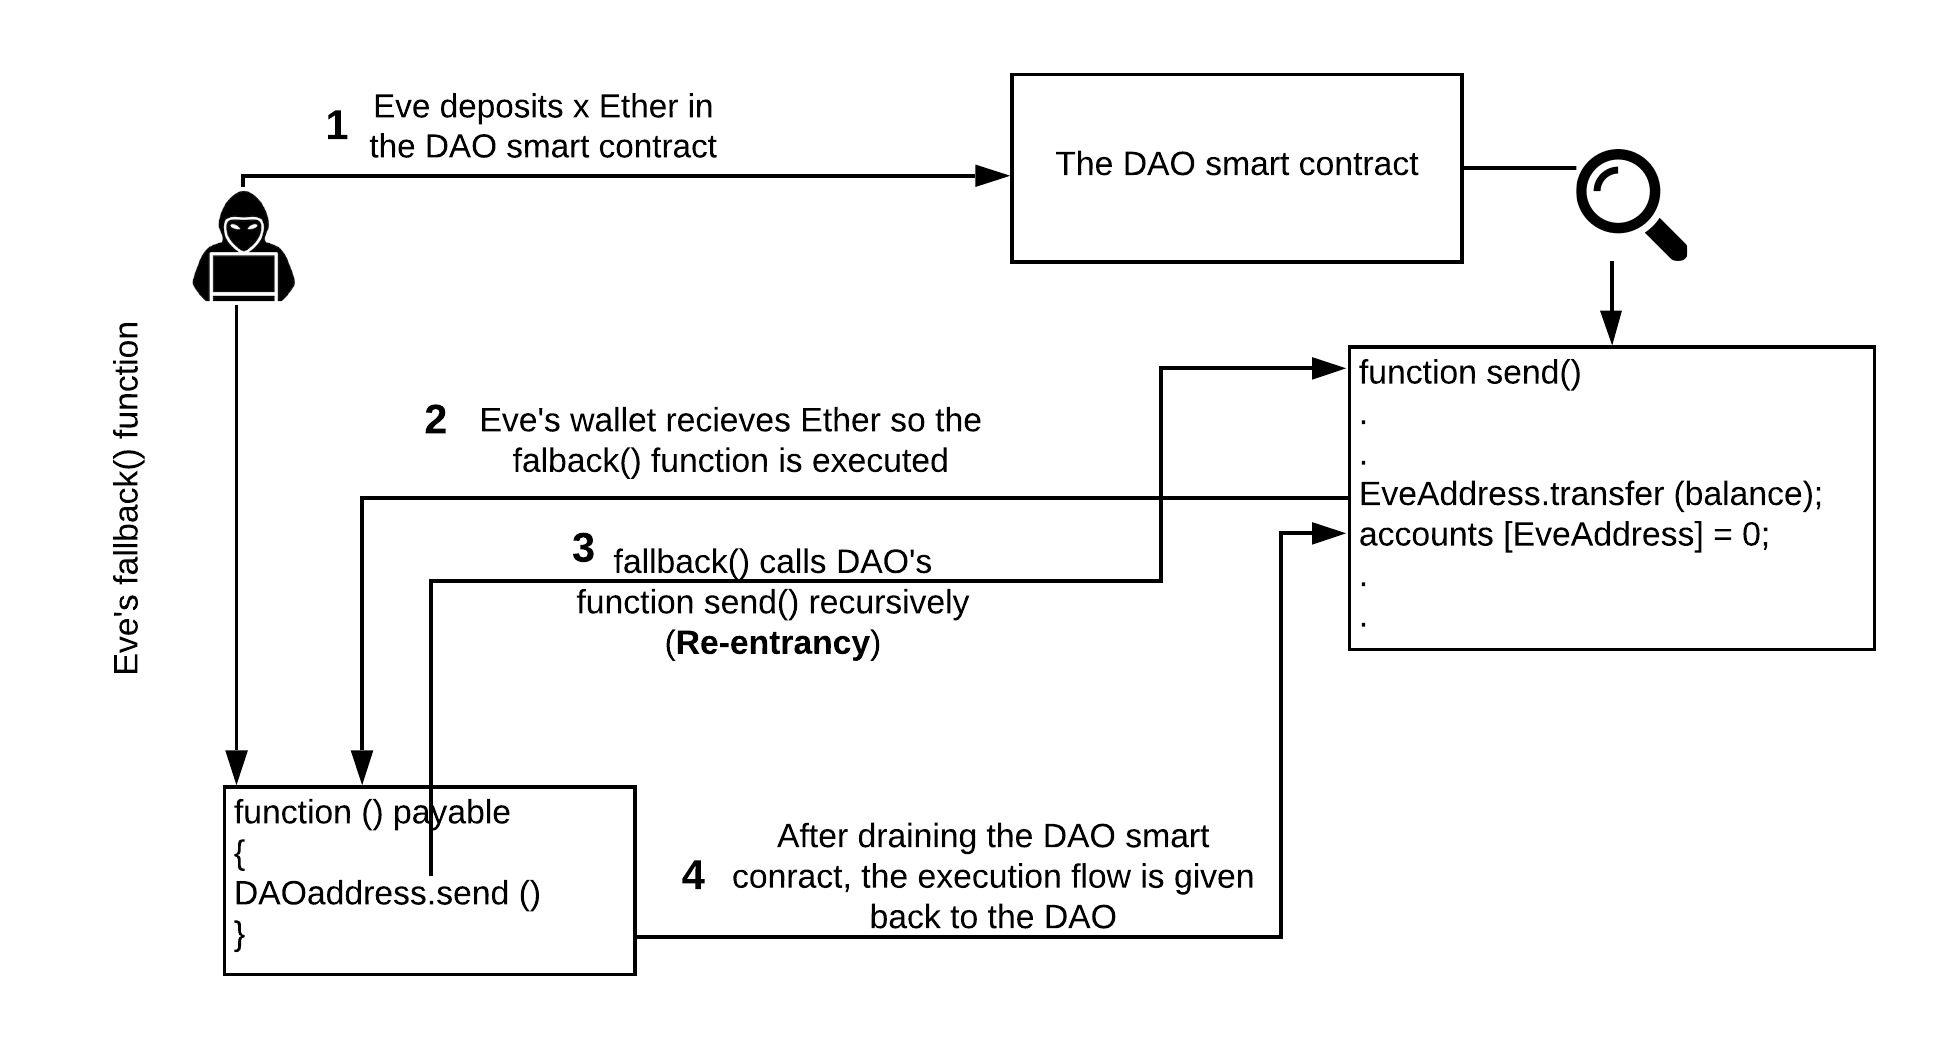
\includegraphics[width=1.0\linewidth]{figures/DAO_flowchart.png}
	\caption{The re-entrancy attack diagram.}
	\label{fig:DAO_flowchart}
\end{figure}


\begin{lstlisting}[basicstyle=\scriptsize\ttfamily,caption={The attacker's malicious smart contract that drains funds from the DAO smart contract.},label={code:attackdao},float]
Import ?browser/SimpleDAO.sol ?;
Contract Attacker 
{
	//assign SimpleDAO contract as dao
	SimpleDAO public dao = SimpleDAO (0x2ae...);
	address owner;
	
	//assign the contract creator as owner
	constructor (Attacker) public {
		owner = msg.sender;
	}
	
	//a fallback() function that receives no data and withdraws funds from SImpleDAO
	function() public payable {
		dao.withdraw (dao.assignedCredit (this)) ;
	}
	
	//attacker sends all the funds to his personal address
	function drainfunds() payable public{
		owner.transfer (address(this).balance);
	}
}
	
\end{lstlisting}


\subsubsection{Attack Mitigation}
Dapp designers and developers can prevent the re-entrancy attack using the following solutions. The Withdraw() function in the victim's smart contract can be locked using the Ethereum's state machine and it can only be executed when it is in \textit{unlocked} state. As it can be seen in (Code~\ref{code:lockdao}, line 12) we can lock the withdraw() function in the first line of the body of the function and unlock it before transferring the funds to the user (see Code~\ref{code:lockdao}, line 17). Thus, if the fallback() function starts recursive calls, it never reaches to the last line of the body of the withdraw() function where we unlock the state again. This prevents the fallback from calling the withdraw() function repeatedly. Maintaining a lock is necessary but not sufficient to prevent the reentrancy attack, DApps developers have to rely on this approach when designing smart contracts (maintaining a lock in Ethereum is not very expensive). Another preventive design decision the Dapp developers need to be aware of is updating the smart contract’s state (user’s balance) before transferring any funds to the msg.sender (user) (Code~\ref{code:lockdao}, line 16). To fully prevent the the re-entrancy attack, the mentioned techniques are necessary yet not sufficient. 

\begin{lstlisting}[basicstyle=\scriptsize\ttfamily,caption={The simplified version of the DAO smart contract that uses the state machine to lock the withdraw() function.},label={code:lockdao},float]
Contract SimpleDAO 
{
	...
	//Possible states of withdraw() function.
	enum <@\textcolor{cyan}{Stages}@> {Opened, Locked} 
	
	Stages stage;
	
	function withdraw (unit amount)
	{	
		require(stage == Stages.Opened);
		stage = Stages.Locked;
		if ( credit[msg.sender] >= amount )
		{	
			credit[msg.sender] -= amount;	
			msg.sender.call.value (amount) () ;
			stage = Stages.Opened;
		}
	}              
}
\end{lstlisting}
The last method which strongly prevents the re-entrancy attack is to limit the amount of Gas that is given to the fallback() function. \textit{Send()} and \textit{Transfer()} are the two Solidity functions that only have 2300 Gas which is only enough for event logging and not any other action. In this case, if the attacker's fallback() function wants to log event it can, but anything else is not doable as the Gas will not be enough.
